% Options for packages loaded elsewhere
\PassOptionsToPackage{unicode}{hyperref}
\PassOptionsToPackage{hyphens}{url}
\PassOptionsToPackage{dvipsnames,svgnames*,x11names*}{xcolor}
%
\documentclass[
]{article}
\usepackage{amsmath,amssymb}
\usepackage{lmodern}
\usepackage{ifxetex,ifluatex}
\ifnum 0\ifxetex 1\fi\ifluatex 1\fi=0 % if pdftex
  \usepackage[T1]{fontenc}
  \usepackage[utf8]{inputenc}
  \usepackage{textcomp} % provide euro and other symbols
\else % if luatex or xetex
  \usepackage{unicode-math}
  \defaultfontfeatures{Scale=MatchLowercase}
  \defaultfontfeatures[\rmfamily]{Ligatures=TeX,Scale=1}
\fi
% Use upquote if available, for straight quotes in verbatim environments
\IfFileExists{upquote.sty}{\usepackage{upquote}}{}
\IfFileExists{microtype.sty}{% use microtype if available
  \usepackage[]{microtype}
  \UseMicrotypeSet[protrusion]{basicmath} % disable protrusion for tt fonts
}{}
\makeatletter
\@ifundefined{KOMAClassName}{% if non-KOMA class
  \IfFileExists{parskip.sty}{%
    \usepackage{parskip}
  }{% else
    \setlength{\parindent}{0pt}
    \setlength{\parskip}{6pt plus 2pt minus 1pt}}
}{% if KOMA class
  \KOMAoptions{parskip=half}}
\makeatother
\usepackage{xcolor}
\IfFileExists{xurl.sty}{\usepackage{xurl}}{} % add URL line breaks if available
\IfFileExists{bookmark.sty}{\usepackage{bookmark}}{\usepackage{hyperref}}
\hypersetup{
  pdftitle={Add Title},
  pdfauthor={Ordinary Leading Students},
  colorlinks=true,
  linkcolor=Maroon,
  filecolor=Maroon,
  citecolor=Blue,
  urlcolor=blue,
  pdfcreator={LaTeX via pandoc}}
\urlstyle{same} % disable monospaced font for URLs
\usepackage[margin=1in]{geometry}
\usepackage{color}
\usepackage{fancyvrb}
\newcommand{\VerbBar}{|}
\newcommand{\VERB}{\Verb[commandchars=\\\{\}]}
\DefineVerbatimEnvironment{Highlighting}{Verbatim}{commandchars=\\\{\}}
% Add ',fontsize=\small' for more characters per line
\usepackage{framed}
\definecolor{shadecolor}{RGB}{248,248,248}
\newenvironment{Shaded}{\begin{snugshade}}{\end{snugshade}}
\newcommand{\AlertTok}[1]{\textcolor[rgb]{0.94,0.16,0.16}{#1}}
\newcommand{\AnnotationTok}[1]{\textcolor[rgb]{0.56,0.35,0.01}{\textbf{\textit{#1}}}}
\newcommand{\AttributeTok}[1]{\textcolor[rgb]{0.77,0.63,0.00}{#1}}
\newcommand{\BaseNTok}[1]{\textcolor[rgb]{0.00,0.00,0.81}{#1}}
\newcommand{\BuiltInTok}[1]{#1}
\newcommand{\CharTok}[1]{\textcolor[rgb]{0.31,0.60,0.02}{#1}}
\newcommand{\CommentTok}[1]{\textcolor[rgb]{0.56,0.35,0.01}{\textit{#1}}}
\newcommand{\CommentVarTok}[1]{\textcolor[rgb]{0.56,0.35,0.01}{\textbf{\textit{#1}}}}
\newcommand{\ConstantTok}[1]{\textcolor[rgb]{0.00,0.00,0.00}{#1}}
\newcommand{\ControlFlowTok}[1]{\textcolor[rgb]{0.13,0.29,0.53}{\textbf{#1}}}
\newcommand{\DataTypeTok}[1]{\textcolor[rgb]{0.13,0.29,0.53}{#1}}
\newcommand{\DecValTok}[1]{\textcolor[rgb]{0.00,0.00,0.81}{#1}}
\newcommand{\DocumentationTok}[1]{\textcolor[rgb]{0.56,0.35,0.01}{\textbf{\textit{#1}}}}
\newcommand{\ErrorTok}[1]{\textcolor[rgb]{0.64,0.00,0.00}{\textbf{#1}}}
\newcommand{\ExtensionTok}[1]{#1}
\newcommand{\FloatTok}[1]{\textcolor[rgb]{0.00,0.00,0.81}{#1}}
\newcommand{\FunctionTok}[1]{\textcolor[rgb]{0.00,0.00,0.00}{#1}}
\newcommand{\ImportTok}[1]{#1}
\newcommand{\InformationTok}[1]{\textcolor[rgb]{0.56,0.35,0.01}{\textbf{\textit{#1}}}}
\newcommand{\KeywordTok}[1]{\textcolor[rgb]{0.13,0.29,0.53}{\textbf{#1}}}
\newcommand{\NormalTok}[1]{#1}
\newcommand{\OperatorTok}[1]{\textcolor[rgb]{0.81,0.36,0.00}{\textbf{#1}}}
\newcommand{\OtherTok}[1]{\textcolor[rgb]{0.56,0.35,0.01}{#1}}
\newcommand{\PreprocessorTok}[1]{\textcolor[rgb]{0.56,0.35,0.01}{\textit{#1}}}
\newcommand{\RegionMarkerTok}[1]{#1}
\newcommand{\SpecialCharTok}[1]{\textcolor[rgb]{0.00,0.00,0.00}{#1}}
\newcommand{\SpecialStringTok}[1]{\textcolor[rgb]{0.31,0.60,0.02}{#1}}
\newcommand{\StringTok}[1]{\textcolor[rgb]{0.31,0.60,0.02}{#1}}
\newcommand{\VariableTok}[1]{\textcolor[rgb]{0.00,0.00,0.00}{#1}}
\newcommand{\VerbatimStringTok}[1]{\textcolor[rgb]{0.31,0.60,0.02}{#1}}
\newcommand{\WarningTok}[1]{\textcolor[rgb]{0.56,0.35,0.01}{\textbf{\textit{#1}}}}
\usepackage{graphicx}
\makeatletter
\def\maxwidth{\ifdim\Gin@nat@width>\linewidth\linewidth\else\Gin@nat@width\fi}
\def\maxheight{\ifdim\Gin@nat@height>\textheight\textheight\else\Gin@nat@height\fi}
\makeatother
% Scale images if necessary, so that they will not overflow the page
% margins by default, and it is still possible to overwrite the defaults
% using explicit options in \includegraphics[width, height, ...]{}
\setkeys{Gin}{width=\maxwidth,height=\maxheight,keepaspectratio}
% Set default figure placement to htbp
\makeatletter
\def\fps@figure{htbp}
\makeatother
\setlength{\emergencystretch}{3em} % prevent overfull lines
\providecommand{\tightlist}{%
  \setlength{\itemsep}{0pt}\setlength{\parskip}{0pt}}
\setcounter{secnumdepth}{-\maxdimen} % remove section numbering
\usepackage{subfig}
\usepackage{bbm}
\ifluatex
  \usepackage{selnolig}  % disable illegal ligatures
\fi

\title{Add Title}
\author{Ordinary Leading Students}
\date{6/02/2021}

\begin{document}
\maketitle

\begin{abstract}
In the following paper we will present a statistical analysis of stroke related data. Our goal will be to predict whether a patient is likely to get stroke based on multiple input parameters like gender, age, various diseases, and smoking status.
Each row in the data provides relevant information about the patient.

After some data cleaning, we plotted some interesting variables of our dataset to get some insight on
the content and structure of our data.
We then proceeded to the analysis. 


**Add info**
\end{abstract}

\section{Data}

We will now load and present our dataset (that can be retrieved at the
following
\href{https://www.kaggle.com/fedesoriano/stroke-prediction-dataset}{link}).\\

\begin{enumerate}
\item id: unique identifier
\item gender: [Male, Female, Other]
\item age: age of the patient
\item hypertension = $\begin{cases} 1 \quad \text{if the patient has hypertension}\\  0 \quad \text{otherwise} \end{cases}$
\item heart\_disease = $\begin{cases} 1 \quad \text{if the patient has a heart disease}\\  0 \quad \text{otherwise} \end{cases}$
\item ever\_married = [Yes, No]
\item work\_type = [children, Govt\_jov, Never\_worked, Private, Self-employed]
\item Residence\_type = [Rural, Urban]
\item avg\_glucose\_level: average glucose level in blood
\item bmi: body mass index
\item smoking\_status = [formerly smoked, never smoked, smokes, Unknown\footnote{The information is unavailable for this patient}]
\item stroke = $\begin{cases} 1 \quad \text{if the patient had a stroke}\\  0 \quad \text{otherwise} \end{cases}$
\end{enumerate}

\hfill\break

\begin{Shaded}
\begin{Highlighting}[]
\CommentTok{\# Load and summarize dataset}
\NormalTok{dataset }\OtherTok{=} \FunctionTok{read.csv}\NormalTok{(}\StringTok{"stroke.csv"}\NormalTok{)}
\FunctionTok{str}\NormalTok{(dataset)}
\end{Highlighting}
\end{Shaded}

\begin{verbatim}
## 'data.frame':    5110 obs. of  12 variables:
##  $ id               : int  9046 51676 31112 60182 1665 56669 53882 10434 27419 60491 ...
##  $ gender           : chr  "Male" "Female" "Male" "Female" ...
##  $ age              : num  67 61 80 49 79 81 74 69 59 78 ...
##  $ hypertension     : int  0 0 0 0 1 0 1 0 0 0 ...
##  $ heart_disease    : int  1 0 1 0 0 0 1 0 0 0 ...
##  $ ever_married     : chr  "Yes" "Yes" "Yes" "Yes" ...
##  $ work_type        : chr  "Private" "Self-employed" "Private" "Private" ...
##  $ Residence_type   : chr  "Urban" "Rural" "Rural" "Urban" ...
##  $ avg_glucose_level: num  229 202 106 171 174 ...
##  $ bmi              : chr  "36.6" "N/A" "32.5" "34.4" ...
##  $ smoking_status   : chr  "formerly smoked" "never smoked" "never smoked" "smokes" ...
##  $ stroke           : int  1 1 1 1 1 1 1 1 1 1 ...
\end{verbatim}

\section{Data Cleaning}

We convert our variables in the right data type and we show the updated
summary.\\

\begin{Shaded}
\begin{Highlighting}[]
\CommentTok{\# Remove id column (useless)}
\NormalTok{dataset}\SpecialCharTok{$}\NormalTok{id }\OtherTok{=} \ConstantTok{NULL}

\CommentTok{\# Convert qualitative variables in factors}
\NormalTok{dataset}\SpecialCharTok{$}\NormalTok{gender          }\OtherTok{=} \FunctionTok{factor}\NormalTok{(dataset}\SpecialCharTok{$}\NormalTok{gender)}
\NormalTok{dataset}\SpecialCharTok{$}\NormalTok{hypertension    }\OtherTok{=} \FunctionTok{factor}\NormalTok{(dataset}\SpecialCharTok{$}\NormalTok{hypertension, }\AttributeTok{levels =} \FunctionTok{c}\NormalTok{(}\DecValTok{0}\NormalTok{,}\DecValTok{1}\NormalTok{), }\AttributeTok{labels =} \FunctionTok{c}\NormalTok{(}\StringTok{"No"}\NormalTok{, }\StringTok{"Yes"}\NormalTok{))}
\NormalTok{dataset}\SpecialCharTok{$}\NormalTok{heart\_disease   }\OtherTok{=} \FunctionTok{factor}\NormalTok{(dataset}\SpecialCharTok{$}\NormalTok{heart\_disease, }\AttributeTok{levels =} \FunctionTok{c}\NormalTok{(}\DecValTok{0}\NormalTok{,}\DecValTok{1}\NormalTok{), }\AttributeTok{labels =} \FunctionTok{c}\NormalTok{(}\StringTok{"No"}\NormalTok{, }\StringTok{"Yes"}\NormalTok{))}
\NormalTok{dataset}\SpecialCharTok{$}\NormalTok{ever\_married    }\OtherTok{=} \FunctionTok{factor}\NormalTok{(dataset}\SpecialCharTok{$}\NormalTok{ever\_married)}
\NormalTok{dataset}\SpecialCharTok{$}\NormalTok{work\_type       }\OtherTok{=} \FunctionTok{factor}\NormalTok{(dataset}\SpecialCharTok{$}\NormalTok{work\_type)}
\NormalTok{dataset}\SpecialCharTok{$}\NormalTok{residence\_type  }\OtherTok{=} \FunctionTok{factor}\NormalTok{(dataset}\SpecialCharTok{$}\NormalTok{Residence\_type)}
\NormalTok{dataset}\SpecialCharTok{$}\NormalTok{smoking\_status  }\OtherTok{=} \FunctionTok{factor}\NormalTok{(dataset}\SpecialCharTok{$}\NormalTok{smoking\_status)}
\NormalTok{dataset}\SpecialCharTok{$}\NormalTok{stroke          }\OtherTok{=} \FunctionTok{factor}\NormalTok{(dataset}\SpecialCharTok{$}\NormalTok{stroke, }\AttributeTok{levels =} \FunctionTok{c}\NormalTok{(}\DecValTok{0}\NormalTok{,}\DecValTok{1}\NormalTok{), }\AttributeTok{labels =} \FunctionTok{c}\NormalTok{(}\StringTok{"No"}\NormalTok{, }\StringTok{"Yes"}\NormalTok{))}

\CommentTok{\# Convert quantitative variable in numeric}
\NormalTok{dataset}\SpecialCharTok{$}\NormalTok{bmi             }\OtherTok{=} \FunctionTok{as.numeric}\NormalTok{(dataset}\SpecialCharTok{$}\NormalTok{bmi)}

\CommentTok{\# Remove duplicate column (due to uppercase)}
\NormalTok{dataset}\SpecialCharTok{$}\NormalTok{Residence\_type  }\OtherTok{=} \ConstantTok{NULL} 

\CommentTok{\# Show dataset summary}
\FunctionTok{str}\NormalTok{(dataset)}
\end{Highlighting}
\end{Shaded}

\begin{verbatim}
## 'data.frame':    5110 obs. of  11 variables:
##  $ gender           : Factor w/ 3 levels "Female","Male",..: 2 1 2 1 1 2 2 1 1 1 ...
##  $ age              : num  67 61 80 49 79 81 74 69 59 78 ...
##  $ hypertension     : Factor w/ 2 levels "No","Yes": 1 1 1 1 2 1 2 1 1 1 ...
##  $ heart_disease    : Factor w/ 2 levels "No","Yes": 2 1 2 1 1 1 2 1 1 1 ...
##  $ ever_married     : Factor w/ 2 levels "No","Yes": 2 2 2 2 2 2 2 1 2 2 ...
##  $ work_type        : Factor w/ 5 levels "children","Govt_job",..: 4 5 4 4 5 4 4 4 4 4 ...
##  $ avg_glucose_level: num  229 202 106 171 174 ...
##  $ bmi              : num  36.6 NA 32.5 34.4 24 29 27.4 22.8 NA 24.2 ...
##  $ smoking_status   : Factor w/ 4 levels "formerly smoked",..: 1 2 2 3 2 1 2 2 4 4 ...
##  $ stroke           : Factor w/ 2 levels "No","Yes": 2 2 2 2 2 2 2 2 2 2 ...
##  $ residence_type   : Factor w/ 2 levels "Rural","Urban": 2 1 1 2 1 2 1 2 1 2 ...
\end{verbatim}

\newpage

\section{ Data Visualization}

We can use different boxplots to visualize possible relations between
our quantitative variables (\textbf{age}, \textbf{bmi} and
\textbf{Average glucose level}) and stroke status.\\

\begin{Shaded}
\begin{Highlighting}[]
\FunctionTok{grid.arrange}\NormalTok{(}\FunctionTok{ggplot}\NormalTok{(dataset, }\FunctionTok{aes}\NormalTok{(}\AttributeTok{x=}\NormalTok{stroke ,}\AttributeTok{y=}\NormalTok{age)) }\SpecialCharTok{+}
              \FunctionTok{geom\_boxplot}\NormalTok{(}\AttributeTok{fill=} \StringTok{"\#FDE725FF"}\NormalTok{, }\AttributeTok{alpha=} \FloatTok{0.7}\NormalTok{), }
            \FunctionTok{ggplot}\NormalTok{(dataset, }\FunctionTok{aes}\NormalTok{(}\AttributeTok{x=}\NormalTok{stroke, }\AttributeTok{y=}\NormalTok{bmi))}\SpecialCharTok{+}
              \FunctionTok{geom\_boxplot}\NormalTok{(}\AttributeTok{fill=} \StringTok{"\#2D708EFF"}\NormalTok{, }\AttributeTok{alpha=} \FloatTok{0.7}\NormalTok{), }
            \FunctionTok{ggplot}\NormalTok{(dataset, }\FunctionTok{aes}\NormalTok{(}\AttributeTok{x=}\NormalTok{stroke, }\AttributeTok{y=}\NormalTok{avg\_glucose\_level))}\SpecialCharTok{+}
              \FunctionTok{geom\_boxplot}\NormalTok{(}\AttributeTok{fill=} \StringTok{"\#440154FF"}\NormalTok{, }\AttributeTok{alpha=} \FloatTok{0.7}\NormalTok{), }
            \AttributeTok{ncol=}\DecValTok{3}\NormalTok{)}
\end{Highlighting}
\end{Shaded}

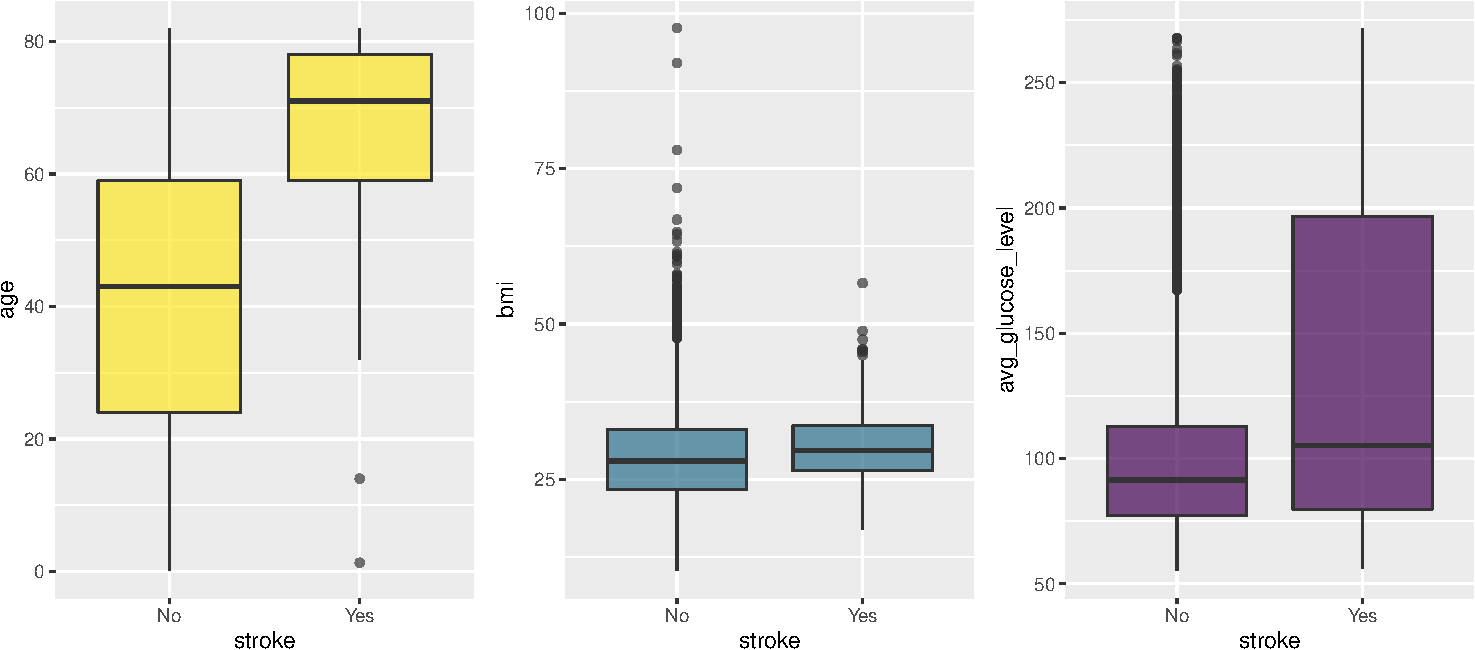
\includegraphics{report_files/figure-latex/unnamed-chunk-4-1.pdf}

From the plots above we can infer the following:

\begin{itemize}
\item \textbf{Age}: older people are more likely to have a stroke.
\item \textbf{Bmi}: there is no evident relation between stroke and bmi.
\item \textbf{Average glucose level}: the higher the level of glucose, the higher the relation with stroke
\end{itemize}

Below we plot a few matrices to visualize possible relations between our
qualitative variables and stroke status.\\

\begin{Shaded}
\begin{Highlighting}[]
\FunctionTok{grid.arrange}\NormalTok{(}\FunctionTok{factors\_plot}\NormalTok{(}\FunctionTok{tidy}\NormalTok{(}\FunctionTok{table}\NormalTok{(dataset }\SpecialCharTok{\%\textgreater{}\%}\NormalTok{ dplyr}\SpecialCharTok{::}\FunctionTok{select}\NormalTok{(stroke,work\_type))), }\AttributeTok{palette=}\StringTok{\textquotesingle{}Blues\textquotesingle{}}\NormalTok{,}
                         \AttributeTok{font\_count\_size=}\DecValTok{4}\NormalTok{, }\AttributeTok{font\_normalized\_size=}\FloatTok{5.1}\NormalTok{, }\AttributeTok{font\_percentages\_size=}\FloatTok{2.5}\NormalTok{,}
                         \AttributeTok{font\_categories\_size=}\DecValTok{10}\NormalTok{), }
            \FunctionTok{factors\_plot}\NormalTok{(}\FunctionTok{tidy}\NormalTok{(}\FunctionTok{table}\NormalTok{(dataset }\SpecialCharTok{\%\textgreater{}\%}\NormalTok{ dplyr}\SpecialCharTok{::}\FunctionTok{select}\NormalTok{(stroke,smoking\_status))), }\AttributeTok{palette=}\StringTok{\textquotesingle{}Greens\textquotesingle{}}\NormalTok{,}
                         \AttributeTok{font\_count\_size=}\DecValTok{4}\NormalTok{, }\AttributeTok{font\_normalized\_size=}\FloatTok{5.1}\NormalTok{, }\AttributeTok{font\_percentages\_size=}\FloatTok{2.5}\NormalTok{,}
                         \AttributeTok{font\_categories\_size=}\DecValTok{10}\NormalTok{),}
            \FunctionTok{factors\_plot}\NormalTok{(}\FunctionTok{tidy}\NormalTok{(}\FunctionTok{table}\NormalTok{(dataset }\SpecialCharTok{\%\textgreater{}\%}\NormalTok{ dplyr}\SpecialCharTok{::}\FunctionTok{select}\NormalTok{(stroke,gender))), }\AttributeTok{palette=}\StringTok{\textquotesingle{}Purples\textquotesingle{}}\NormalTok{,}
                         \AttributeTok{font\_count\_size=}\DecValTok{4}\NormalTok{, }\AttributeTok{font\_normalized\_size=}\FloatTok{5.1}\NormalTok{, }\AttributeTok{font\_percentages\_size=}\FloatTok{2.5}\NormalTok{,}
                         \AttributeTok{font\_categories\_size=}\DecValTok{10}\NormalTok{),}
            \AttributeTok{ncol=}\DecValTok{3}\NormalTok{, }\AttributeTok{nrow=}\DecValTok{1}\NormalTok{)}
\end{Highlighting}
\end{Shaded}

\begin{center}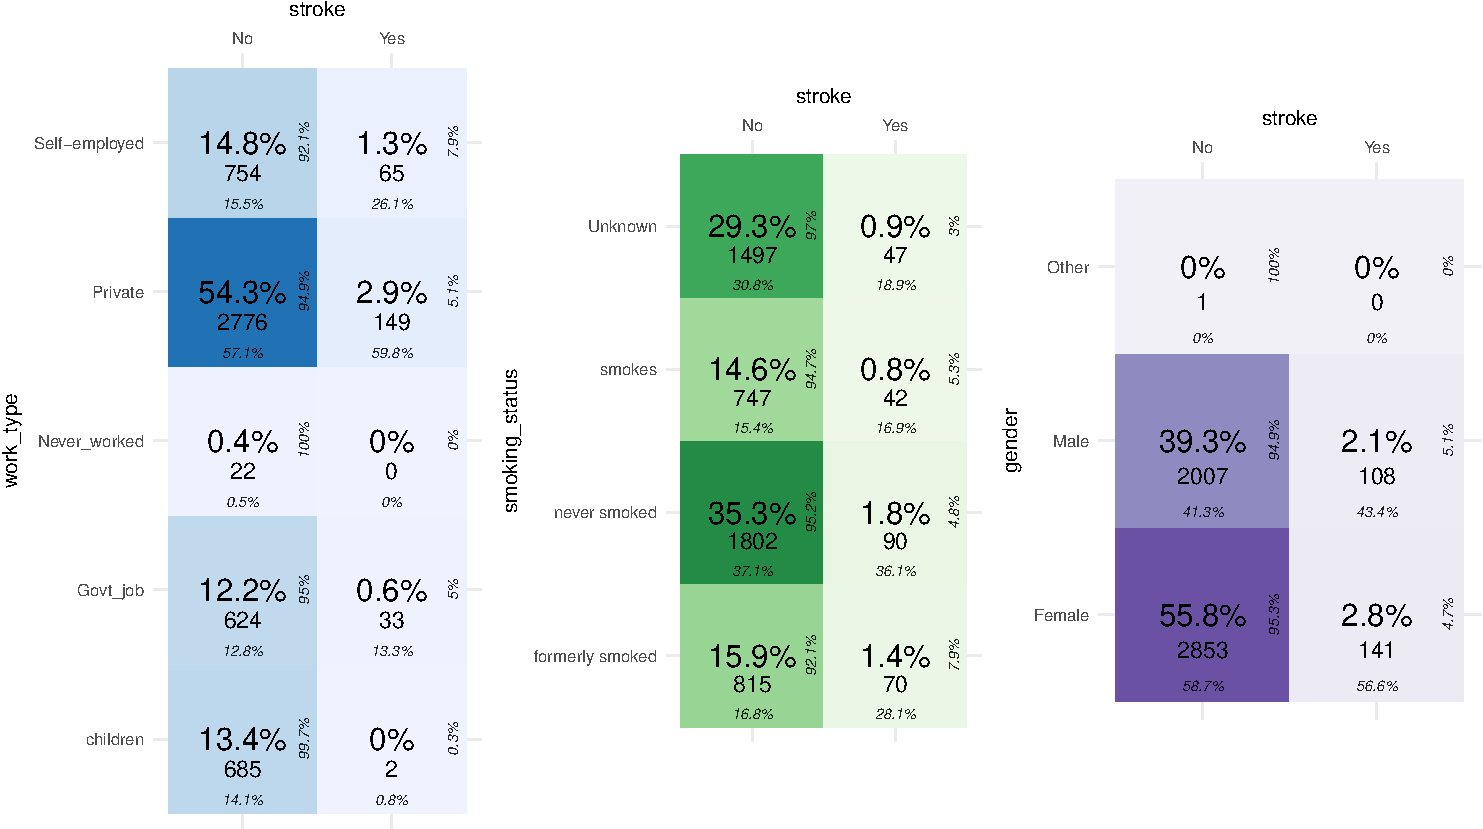
\includegraphics{report_files/figure-latex/unnamed-chunk-5-1} \end{center}

\begin{Shaded}
\begin{Highlighting}[]
\FunctionTok{grid.arrange}\NormalTok{(}\FunctionTok{factors\_plot}\NormalTok{(}\FunctionTok{tidy}\NormalTok{(}\FunctionTok{table}\NormalTok{(dataset }\SpecialCharTok{\%\textgreater{}\%}\NormalTok{ dplyr}\SpecialCharTok{::}\FunctionTok{select}\NormalTok{(stroke,hypertension))), }\AttributeTok{palette=}\StringTok{\textquotesingle{}Greens\textquotesingle{}}\NormalTok{,}
                         \AttributeTok{font\_count\_size=}\FloatTok{3.5}\NormalTok{, }\AttributeTok{font\_normalized\_size=}\DecValTok{5}\NormalTok{, }\AttributeTok{font\_percentages\_size=}\FloatTok{2.5}\NormalTok{,}
                         \AttributeTok{font\_categories\_size=}\DecValTok{10}\NormalTok{), }
            \FunctionTok{factors\_plot}\NormalTok{(}\FunctionTok{tidy}\NormalTok{(}\FunctionTok{table}\NormalTok{(dataset }\SpecialCharTok{\%\textgreater{}\%}\NormalTok{ dplyr}\SpecialCharTok{::}\FunctionTok{select}\NormalTok{(stroke,heart\_disease))), }\AttributeTok{palette=}\StringTok{\textquotesingle{}Blues\textquotesingle{}}\NormalTok{,}
                         \AttributeTok{font\_count\_size=}\FloatTok{3.5}\NormalTok{, }\AttributeTok{font\_normalized\_size=}\DecValTok{5}\NormalTok{, }\AttributeTok{font\_percentages\_size=}\FloatTok{2.5}\NormalTok{,}
                         \AttributeTok{font\_categories\_size=}\DecValTok{10}\NormalTok{), }
            \FunctionTok{factors\_plot}\NormalTok{(}\FunctionTok{tidy}\NormalTok{(}\FunctionTok{table}\NormalTok{(dataset }\SpecialCharTok{\%\textgreater{}\%}\NormalTok{ dplyr}\SpecialCharTok{::}\FunctionTok{select}\NormalTok{(stroke,residence\_type))), }\AttributeTok{palette=}\StringTok{\textquotesingle{}Purples\textquotesingle{}}\NormalTok{,}
                         \AttributeTok{font\_count\_size=}\FloatTok{3.5}\NormalTok{, }\AttributeTok{font\_normalized\_size=}\DecValTok{5}\NormalTok{, }\AttributeTok{font\_percentages\_size=}\FloatTok{2.5}\NormalTok{,}
                         \AttributeTok{font\_categories\_size=}\DecValTok{10}\NormalTok{),}
            \FunctionTok{factors\_plot}\NormalTok{(}\FunctionTok{tidy}\NormalTok{(}\FunctionTok{table}\NormalTok{(dataset }\SpecialCharTok{\%\textgreater{}\%}\NormalTok{ dplyr}\SpecialCharTok{::}\FunctionTok{select}\NormalTok{(stroke,ever\_married))), }\AttributeTok{palette=}\StringTok{\textquotesingle{}Oranges\textquotesingle{}}\NormalTok{,}
                         \AttributeTok{font\_count\_size=}\FloatTok{3.5}\NormalTok{, }\AttributeTok{font\_normalized\_size=}\DecValTok{5}\NormalTok{, }\AttributeTok{font\_percentages\_size=}\FloatTok{2.5}\NormalTok{,}
                         \AttributeTok{font\_categories\_size=}\DecValTok{10}\NormalTok{),}
            \AttributeTok{ncol=}\DecValTok{2}\NormalTok{, }\AttributeTok{nrow=}\DecValTok{2}\NormalTok{)}
\end{Highlighting}
\end{Shaded}

\begin{center}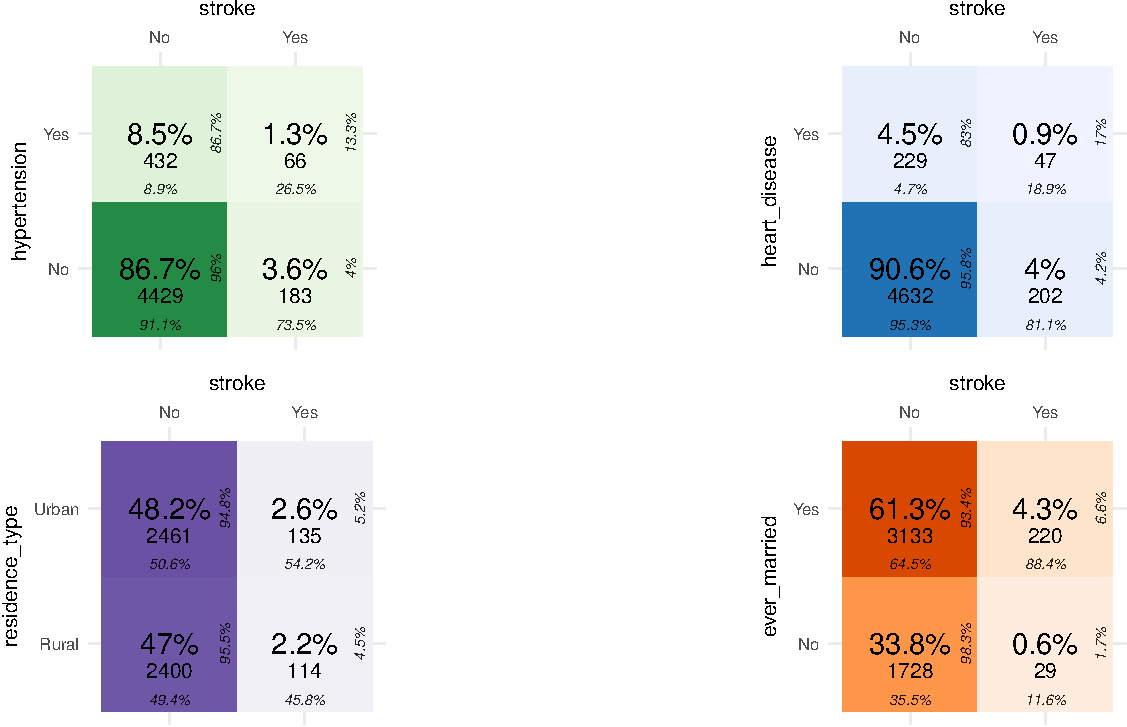
\includegraphics{report_files/figure-latex/unnamed-chunk-6-1} \end{center}

And we can finally show \textbf{qualitative} and \textbf{quantitative}
correlations.

\begin{Shaded}
\begin{Highlighting}[]
\NormalTok{qualitative\_vars }\OtherTok{=} \FunctionTok{c}\NormalTok{(}\StringTok{\textquotesingle{}gender\textquotesingle{}}\NormalTok{, }\StringTok{\textquotesingle{}hypertension\textquotesingle{}}\NormalTok{, }\StringTok{\textquotesingle{}heart\_disease\textquotesingle{}}\NormalTok{, }\StringTok{\textquotesingle{}ever\_married\textquotesingle{}}\NormalTok{,}
                      \StringTok{\textquotesingle{}work\_type\textquotesingle{}}\NormalTok{, }\StringTok{\textquotesingle{}smoking\_status\textquotesingle{}}\NormalTok{, }\StringTok{\textquotesingle{}residence\_type\textquotesingle{}}\NormalTok{)}
\FunctionTok{plot}\NormalTok{(}\FunctionTok{GKtauDataframe}\NormalTok{(dataset }\SpecialCharTok{\%\textgreater{}\%}\NormalTok{ dplyr}\SpecialCharTok{::}\FunctionTok{select}\NormalTok{(}\FunctionTok{all\_of}\NormalTok{(qualitative\_vars))))}
\end{Highlighting}
\end{Shaded}

\begin{center}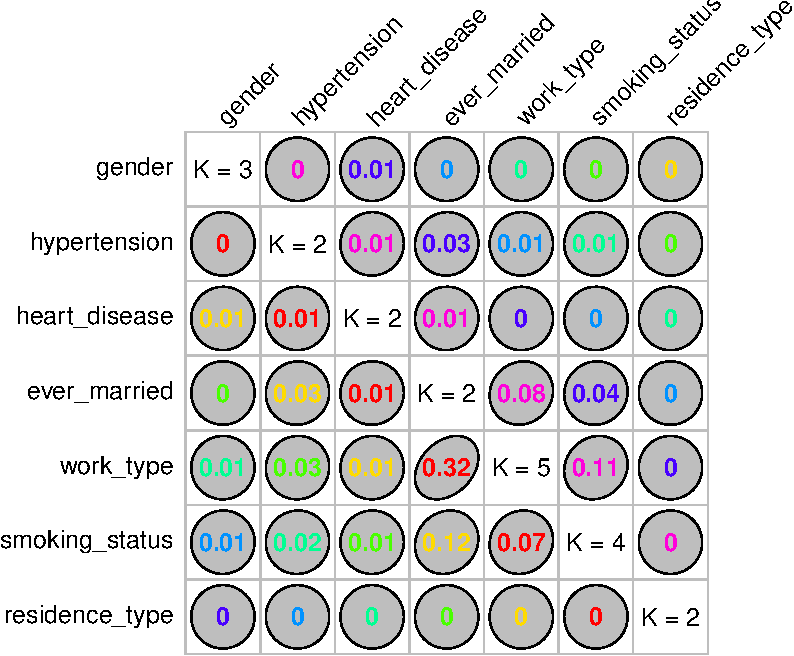
\includegraphics{report_files/figure-latex/unnamed-chunk-7-1} \end{center}

\begin{Shaded}
\begin{Highlighting}[]
\CommentTok{\# }\AlertTok{TODO}\CommentTok{ find a way to plot table and image side{-}by{-}side}

\NormalTok{quantitative\_vars }\OtherTok{=} \FunctionTok{c}\NormalTok{(}\StringTok{\textquotesingle{}age\textquotesingle{}}\NormalTok{, }\StringTok{\textquotesingle{}avg\_glucose\_level\textquotesingle{}}\NormalTok{, }\StringTok{\textquotesingle{}bmi\textquotesingle{}}\NormalTok{)}

\NormalTok{corr }\OtherTok{\textless{}{-}} \FunctionTok{rcorr}\NormalTok{(}\FunctionTok{as.matrix}\NormalTok{(dataset }\SpecialCharTok{\%\textgreater{}\%}\NormalTok{ dplyr}\SpecialCharTok{::}\FunctionTok{select}\NormalTok{(}\FunctionTok{all\_of}\NormalTok{(quantitative\_vars))))}

\FunctionTok{corrplot}\NormalTok{(corr}\SpecialCharTok{$}\NormalTok{r, }\AttributeTok{type =} \StringTok{"upper"}\NormalTok{, }\AttributeTok{tl.col =} \StringTok{"black"}\NormalTok{, }\AttributeTok{tl.srt =} \DecValTok{45}\NormalTok{)}
\end{Highlighting}
\end{Shaded}

\begin{center}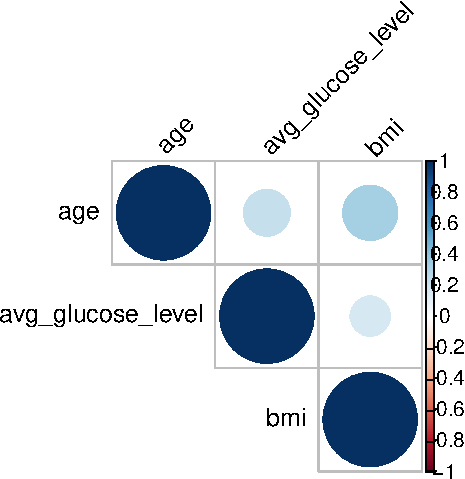
\includegraphics{report_files/figure-latex/unnamed-chunk-8-1} \end{center}

\section{Data Manipulation}

In order to facilitate our work, we removed the level \textbf{other}
from the variable gender and the level \textbf{never\_worked} from the
variable work\_type, since they are not relevant for the analysis.\\

\begin{Shaded}
\begin{Highlighting}[]
\CommentTok{\# Remove rows}
\NormalTok{dataset }\OtherTok{=}\NormalTok{ dataset }\SpecialCharTok{\%\textgreater{}\%}
          \FunctionTok{filter}\NormalTok{(gender }\SpecialCharTok{!=} \StringTok{\textquotesingle{}Other\textquotesingle{}}\NormalTok{) }\SpecialCharTok{\%\textgreater{}\%}
          \FunctionTok{filter}\NormalTok{(work\_type }\SpecialCharTok{!=} \StringTok{\textquotesingle{}Never\_worked\textquotesingle{}}\NormalTok{)}

\CommentTok{\# Remove related levels}
\NormalTok{dataset }\OtherTok{=} \FunctionTok{droplevels}\NormalTok{(dataset)}
\end{Highlighting}
\end{Shaded}

We now have to address NA values:

\begin{Shaded}
\begin{Highlighting}[]
\CommentTok{\# Check for NA in all columns}
\ControlFlowTok{for}\NormalTok{ (col\_name }\ControlFlowTok{in} \FunctionTok{colnames}\NormalTok{(dataset))\{}
   \ControlFlowTok{if}\NormalTok{ (}\FunctionTok{anyNA}\NormalTok{(dataset[[col\_name]]))}
    \FunctionTok{print}\NormalTok{(}\FunctionTok{paste}\NormalTok{(col\_name, }\StringTok{\textquotesingle{}{-}\textgreater{} \textquotesingle{}}\NormalTok{, }\FunctionTok{sum}\NormalTok{(}\FunctionTok{is.na}\NormalTok{(dataset[[col\_name]])), }\StringTok{\textquotesingle{} NA\textquotesingle{}}\NormalTok{))}
\NormalTok{\}}
\end{Highlighting}
\end{Shaded}

\begin{verbatim}
## [1] "bmi ->  201  NA"
\end{verbatim}

We notice that we have 201 NA just in the \textbf{bmi} variable. In
order to avoid losing these rows, given that we already have a small
dataset, we will predict their values using a fitted tree.\\

\begin{Shaded}
\begin{Highlighting}[]
\CommentTok{\# Define test set as set with missing data}
\NormalTok{missing\_index }\OtherTok{\textless{}{-}} \FunctionTok{which}\NormalTok{(}\FunctionTok{is.na}\NormalTok{(dataset}\SpecialCharTok{$}\NormalTok{bmi))}

\NormalTok{test\_set }\OtherTok{\textless{}{-}}\NormalTok{ dataset[missing\_index,]}
\NormalTok{train\_set }\OtherTok{\textless{}{-}}\NormalTok{ dataset[}\SpecialCharTok{{-}}\FunctionTok{c}\NormalTok{(missing\_index),]}

\CommentTok{\# Fit the tree}
\NormalTok{tree }\OtherTok{=}\NormalTok{ caret}\SpecialCharTok{::}\FunctionTok{train}\NormalTok{(bmi }\SpecialCharTok{\textasciitilde{}}\NormalTok{ ., }
                    \AttributeTok{data=}\NormalTok{train\_set, }
                    \AttributeTok{method=}\StringTok{"rpart"}\NormalTok{, }
                    \AttributeTok{trControl =} \FunctionTok{trainControl}\NormalTok{(}\AttributeTok{method =} \StringTok{"cv"}\NormalTok{))}

\CommentTok{\# Replace missing data with predicted data}
\NormalTok{bmi\_pred }\OtherTok{\textless{}{-}} \FunctionTok{predict}\NormalTok{(tree, }\AttributeTok{newdata =}\NormalTok{ test\_set)}
\NormalTok{dataset[missing\_index, }\StringTok{\textquotesingle{}bmi\textquotesingle{}}\NormalTok{] }\OtherTok{\textless{}{-}}\NormalTok{ bmi\_pred}

\CommentTok{\# clean global environment}
\FunctionTok{rm}\NormalTok{(test\_set, train\_set, tree, bmi\_pred, missing\_index)}
\end{Highlighting}
\end{Shaded}

\section{Statistical Model}

We will now begin splitting our dataset in train/test.\\

\begin{Shaded}
\begin{Highlighting}[]
\CommentTok{\# Set a fixed seed in order to have reproducible results}
\FunctionTok{set.seed}\NormalTok{(}\DecValTok{36}\NormalTok{) }\CommentTok{\# Answer to the Ultimate Question of Life, the Universe, and Everything}

\CommentTok{\# 60{-}40 split}
\NormalTok{split\_train\_test }\OtherTok{\textless{}{-}} \FunctionTok{createDataPartition}\NormalTok{(}\AttributeTok{y =}\NormalTok{ dataset}\SpecialCharTok{$}\NormalTok{stroke, }\AttributeTok{p=}\FloatTok{0.6}\NormalTok{, }\AttributeTok{list =}\NormalTok{ F)}
\NormalTok{train }\OtherTok{\textless{}{-}}\NormalTok{ dataset[split\_train\_test,]}
\NormalTok{test }\OtherTok{\textless{}{-}}\NormalTok{  dataset[}\SpecialCharTok{{-}}\NormalTok{split\_train\_test,]}

\FunctionTok{table}\NormalTok{(test}\SpecialCharTok{$}\NormalTok{stroke)}
\end{Highlighting}
\end{Shaded}

\begin{verbatim}
## 
##   No  Yes 
## 1935   99
\end{verbatim}

\subsection{SMOTE algorithm}

Since our dataset has a problem of under sampling, we will use the SMOTE
algorithm to create synthetic new data. \textbf{ADD SMOTE EXPLANATION}\\

\begin{Shaded}
\begin{Highlighting}[]
\CommentTok{\# New smote algo}
\NormalTok{train\_smoted }\OtherTok{\textless{}{-}} \FunctionTok{SMOTE\_NC}\NormalTok{(train, }\StringTok{"stroke"}\NormalTok{, }\AttributeTok{k =} \DecValTok{2}\NormalTok{)}
\end{Highlighting}
\end{Shaded}

\begin{verbatim}
## Variables are continous and categorical, SMOTE_NC could be used.
\end{verbatim}

\begin{Shaded}
\begin{Highlighting}[]
\CommentTok{\# Now we have a balanced dataset}
\FunctionTok{table}\NormalTok{(train\_smoted}\SpecialCharTok{$}\NormalTok{stroke)}
\end{Highlighting}
\end{Shaded}

\begin{verbatim}
## 
##   No  Yes 
## 2903 2903
\end{verbatim}

\subsection{Logistic Regression}

We perform a logistic regression using

\item

\textbf{stroke} as the dependent variable and the rest of the data as
independent variables in order to see if we find some significant
relationships.

\begin{Shaded}
\begin{Highlighting}[]
\NormalTok{Logit }\OtherTok{\textless{}{-}} \FunctionTok{glm}\NormalTok{(stroke}\SpecialCharTok{\textasciitilde{}}\NormalTok{., }\AttributeTok{data=}\NormalTok{train, }\AttributeTok{family =} \FunctionTok{binomial}\NormalTok{(}\AttributeTok{link =} \StringTok{"logit"}\NormalTok{))}
\FunctionTok{summary}\NormalTok{(Logit)}
\end{Highlighting}
\end{Shaded}

\begin{verbatim}
## 
## Call:
## glm(formula = stroke ~ ., family = binomial(link = "logit"), 
##     data = train)
## 
## Deviance Residuals: 
##     Min       1Q   Median       3Q      Max  
## -1.0488  -0.3241  -0.1728  -0.0890   3.3768  
## 
## Coefficients:
##                             Estimate Std. Error z value Pr(>|z|)    
## (Intercept)                -7.039011   1.092996  -6.440 1.19e-10 ***
## genderMale                 -0.045630   0.183505  -0.249   0.8036    
## age                         0.073888   0.007312  10.105  < 2e-16 ***
## hypertensionYes             0.450017   0.206994   2.174   0.0297 *  
## heart_diseaseYes           -0.004686   0.275093  -0.017   0.9864    
## ever_marriedYes            -0.211479   0.284478  -0.743   0.4572    
## work_typeGovt_job          -0.684161   1.143519  -0.598   0.5496    
## work_typePrivate           -0.490756   1.124343  -0.436   0.6625    
## work_typeSelf-employed     -0.759294   1.149727  -0.660   0.5090    
## avg_glucose_level           0.003381   0.001555   2.174   0.0297 *  
## bmi                         0.003168   0.014140   0.224   0.8227    
## smoking_statusnever smoked  0.012950   0.230298   0.056   0.9552    
## smoking_statussmokes        0.282582   0.287329   0.983   0.3254    
## smoking_statusUnknown       0.012833   0.274623   0.047   0.9627    
## residence_typeUrban         0.062733   0.177745   0.353   0.7241    
## ---
## Signif. codes:  0 '***' 0.001 '**' 0.01 '*' 0.05 '.' 0.1 ' ' 1
## 
## (Dispersion parameter for binomial family taken to be 1)
## 
##     Null deviance: 1196.48  on 3052  degrees of freedom
## Residual deviance:  961.64  on 3038  degrees of freedom
## AIC: 991.64
## 
## Number of Fisher Scoring iterations: 8
\end{verbatim}

The only significant variables are \textbf{age},\textbf{hypertension}
and \textbf{average glucose level}, which have a positive impact on the
increase of the logit probability.

\subsection{Confusion Matrix and Statistics}

\begin{Shaded}
\begin{Highlighting}[]
\NormalTok{lr\_prob1 }\OtherTok{\textless{}{-}} \FunctionTok{predict}\NormalTok{(Logit, }\AttributeTok{newdata =}\NormalTok{ test)}

\CommentTok{\# error with the for loop}

\CommentTok{\#lr\_preds\_test \textless{}{-} c(0,0,0,0,0,0,0,0,0)}
\CommentTok{\#i\textless{}{-}1}
\CommentTok{\# for (thresh in seq(0.25,0.35,0.05))\{}
\CommentTok{\#   lr\_pred \textless{}{-} ifelse(lr\_prob1 \textgreater{} thresh,1,0)}
\CommentTok{\#   cm \textless{}{-} table(}
\CommentTok{\#     as.factor(lr\_pred),}
\CommentTok{\#     as.factor(test$stroke)}
\CommentTok{\#   )[2:1, 2:1]}
\CommentTok{\#   lr\_preds\_test[i] \textless{}{-} F\_meas(cm) \# f1 score}
\CommentTok{\#  i\textless{}{-}i+1}
\CommentTok{\# \}}
\CommentTok{\# names(lr\_preds\_test) \textless{}{-} seq(0.25,0.35,0.05)}
\CommentTok{\#   }
\CommentTok{\# }
\CommentTok{\# lr\_preds\_test}
\CommentTok{\# lr\_pred \textless{}{-} as.numeric(ifelse(lr\_prob1 \textgreater{} 0.3,"1","0"))}
\CommentTok{\# tb \textless{}{-} table(Predicted = lr\_pred, Actual = test$stroke)[2:1, 2:1]}
\CommentTok{\# tb}

\CommentTok{\#salini conf matrix}
\CommentTok{\# error when knitting}

\CommentTok{\#lr\_pred1 \textless{}{-} ifelse(lr\_prob1 \textgreater{} 0.65,"1","0")}

\CommentTok{\#confusionMatrix(}
\CommentTok{\#as.factor(lr\_pred1),}
\CommentTok{\#  as.factor(test$stroke),}
\CommentTok{\#  positive = "0" }
\CommentTok{\#)}
\end{Highlighting}
\end{Shaded}

\subsection{ROC Curve}

\begin{Shaded}
\begin{Highlighting}[]
\CommentTok{\#error when knitting}

\NormalTok{test\_roc }\OtherTok{\textless{}{-}} \FunctionTok{roc}\NormalTok{(}\FunctionTok{as.numeric}\NormalTok{(test}\SpecialCharTok{$}\NormalTok{stroke)}\SpecialCharTok{\textasciitilde{}}\NormalTok{lr\_prob1 , }\AttributeTok{plot =} \ConstantTok{TRUE}\NormalTok{, }\AttributeTok{print.auc =} \ConstantTok{TRUE}\NormalTok{,}\AttributeTok{percent=}\ConstantTok{TRUE}\NormalTok{, }\AttributeTok{ci=}\ConstantTok{TRUE}\NormalTok{)}
\end{Highlighting}
\end{Shaded}

\begin{verbatim}
## Setting levels: control = 1, case = 2
\end{verbatim}

\begin{verbatim}
## Setting direction: controls < cases
\end{verbatim}

\includegraphics{report_files/figure-latex/unnamed-chunk-16-1.pdf}

\end{document}
